%!TEX root = ./main.tex
\section{Case Study on Expressiveness}
\label{sec:cases}

In this section, we present several examples to demonstrate the expressive power of our approach.

\begin{figure*}[t]
\centering
\begin{subfigure}{.3\linewidth}
	\begin{spacing}{0.5}
		\begin{flushleft}
			{\scriptsize
			\begin{Codes}
			\qquad (S (K (S I)) K xx yy)\\
			\OneStep{ (((K (S I)) xx (K xx)) yy)}\\
			\OneStep{ (((S I) (K xx)) yy)}\\
			\OneStep{ (I yy ((K xx) yy))}\\
			\OneStep{ (yy ((K xx) yy))}\\
			\OneStep{ (yy xx)}\\
			\end{Codes}
			}
		\end{flushleft}
	\end{spacing}

	\caption{Example of SKI}
	\label{fig:SKI}
\end{subfigure}
\begin{subfigure}{.3\linewidth}
	\begin{spacing}{0.5}
		\begin{flushleft}
			{\scriptsize
			\begin{Codes}
			    (let x 2 (Hygienicadd 1 x))\\
			\OneStep{ (Hygienicadd 1 2)}\\
			\OneStep{ (+ 1 2)}\\
			\OneStep{ 3}\\[2.25em]

			\end{Codes}

			}
		\end{flushleft}

	\end{spacing}

	\caption{Example of \m{Hygienicadd}}
	\label{fig:hygienicadd}
\end{subfigure}
\begin{subfigure}{.25\linewidth}
	\begin{spacing}{0.5}
		\begin{flushleft}
			{\scriptsize
			\begin{Codes}
			    (Odd 2)\\
			\OneStep{ (Even (- 2 1))}\\
			\OneStep{ (Even 1)}\\
			\OneStep{ (Odd (- 1 1))}\\
			\OneStep{ (Odd 0)}\\
			\OneStep{ \#f}\\
			\end{Codes}
			}
		\end{flushleft}

	\end{spacing}

	\caption{Example of \m{Odd} and \m{Even}}
	\label{fig:oddeven}
\end{subfigure}
%newline
\begin{subfigure}{.4\linewidth}
		\begin{flushleft}
			{\scriptsize
			% \begin{Codes}
				\quad\;\;\;\Code{ (Map ($\lambda$ (x) (+ x 1)) (cons 1 (list 2)))}\\
			\OneStep{ \Code{ (Map ($\lambda$ (x) (+ x 1)) (list 1 2))}}\\
			\OneStep{ \Code{ (cons 2 (Map ($\lambda$ (x) (+ 1 x)) (list 2)))}}\\
			\OneStep{ \Code{ (cons 2 (cons 3 (Map ($\lambda$ (x) (+ 1 x)) (list))))}}\\
			\OneStep{ \Code{ (cons 2 (cons 3 (list)))}}\\
			\OneStep{ \Code{ (cons 2 (list 3))}}\\
			\OneStep{ \Code{ (list 2 3)}}\\[2em]
			% \end{Codes}
			}
		\end{flushleft}


	\caption{Example of \m{Map}}
	\label{fig:Map}
\end{subfigure}
\begin{subfigure}{.5\linewidth}
		\begin{flushleft}
			{\scriptsize
			\quad\;\;\;\Code{ (Filter ($\lambda$ (x) (and (> x 1) (< x 4))) (list 1 2 3 4))}\\
			\OneStep{ \Code{ (Filter ($\lambda$ (x) (and (> x 1) (< x 4))) (list 2 3 4))}}\\
			\OneStep{ \Code{ (cons 2 (Filter ($\lambda$ (x) (and (> x 1) (< x 4))) (list 3 4)))}}\\
			\OneStep{ \Code{ (cons 2 (cons 3 (Filter ($\lambda$ (x) (and (> x 1) (< x 4))) (list 4))))}}\\
			\OneStep{ \Code{ (cons 2 (cons 3 (Filter ($\lambda$ (x) (and (> x 1) (< x 4))) (list))))}}\\
			\OneStep{ \Code{ (cons 2 (cons 3 (list)))}}\\
			\OneStep{ \Code{ (cons 2 (list 3))}}\\
			\OneStep{ \Code{ (list 2 3)}}

			}
		\end{flushleft}

	\caption{Example of \m{Filter}}
	\label{fig:Filter}
\end{subfigure}

\caption{Resugaring Examples}
\label{fig:resugaring}
\end{figure*}


\subsection{Simple Sugars}
\label{mark:simple}

We construct some simple syntactic sugars and try it on our tool. Some sugars are inspired by the first work of resugaring \cite{resugaring}.
Take an SKI combinator syntactic sugar as an example. We can regard \m{S} as an expression headed with S, without sub-expression. And for showing a concise result, we add the call-by-need lambda calculus in the core language for this example.
\[
\begin{array}{l}
\drule{\m{S}}{\Code{($\lambda_N$ ($x_1$ $x_2$ $x_3$) ($x_1$ $x_2$ ($x_1$ $x_3$)))}}\\
\drule{\m{K}}{\Code{($\lambda_N$ ($x_1$ $x_2$) $x_1$)}}\\
\drule{\m{I}}{\Code{($\lambda_N$ ($x$) $x$)}}
\end{array}
\]




Although SKI combinator calculus is a reduced version of lambda calculus, we can construct combinators' sugars based on call-by-need lambda calculus in our core language. For the sugar program \Code{(S (K (S I)) K xx yy)}, we get the resugaring sequences as Fig.  \ref{fig:SKI}. Here the sugars contain no sub-expression, then the sugar should just desugar to the core expression. It is interesting that the sugar without sub-expressions (written by lambda calculus) and the sugar with sub-expressions will behave differently. For example, in this case, we can write the sugar as \Code{(S e e e)} and so on, then the sugar may not have to be expanded. Moreover, we can use this difference to force a syntactic sugar desugared using call-by-need lambda calculus. See if we want a sugar \m{ForceAnd} which does not
want to use the context rules of \m{if} to getting the resugaring sequence, we can just write the following sugar.

\[
\drule{\Code{ForceAnd}}{\Code{($\lambda_N$ ($x_1$ $x_2$) (if $x_1$ $x_2$ \false))}}
\]



\ignore{
  For the existing approach, the sugar expression should firstly desugar to
\begin{Codes}
((lambdaN (x1 x2 x3) (x1 x3 (x2 x3)))
  ((lambdaN (x1 x2) x1)
   ((lambdaN  (x1 x2 x3) (x1 x3 (x2 x3)))
    (lambdaN (x) x)))
  (lambdaN (x1 x2) x1)
  xx yy)
\end{Codes}
\reduce{can be removed}

Then in our core language, the execution of expanded expression will contain 33 reduction steps in our implementation. For each step, there will be many attempts to match and substitute the syntactic sugars to resugar the expression. It will omit more steps for a larger expression.
}


\subsection{Hygienic Sugars}
\label{mark:hygienic}


The second work \cite{hygienic} of existing resugaring approach mainly processes hygienic sugar compared to the first work. It uses a DAG to represent the expression. However, hygiene is not hard to be handled by our lazy desugaring strategy. Our algorithm can easily process hygienic sugar without a special data structure.
A typical hygienic problem is as the following example.
\[
\drule{\Code{(Hygienicadd $e_1$ $e_2$)}}{\Code{(let ((x $e_1$)) (+ x $e_2$))}}
\]
% \begin{Codes}
% 	(Hygienicadd e1 e2) \DeStep{ (let ((x e1)) (+ x e2))}
% \end{Codes}
For the existing resugaring approach, if we want to get sequences of \Code{(let (x 2) (Hygienicadd 1 x))}, it will firstly desugar to \Code{(let (x 2) (let x 1 (+ x x)))}, which is awful because the two $x$ in \Code{(+ x x)} should be bound to different values. So the existing hygienic resugaring approach uses abstract syntax DAG to distinct different \m{x} in the desugared expression. But for our approach based on lazy desugaring, the \m{Hygienicadd} sugar does not have to expand until necessary, thus, getting resugaring sequences as Fig.  \ref{fig:hygienicadd} based on a non-hygienic transformer system. We will discuss hygienic problem in Section \ref{mark:hygiene}.


% The lazy desugaring is also convenient for achieving hygiene for non-hygienic core language. For example, \Code{(let x 1 (+ x (let x 2 (+ x 1))))} may be reduced to \Code{(+ 1 (let 1 2 (+ 1 1)))} by a simple core language whose \Code{let} expression does not handle cases like that. But by writing a sugar (not syntactic sugar in the usual sense, because we do not want it to behave as \m{let}) \m{Let}
% \[\drule{\Code{(Let~$e_1$~$e_2$~$e_3$)}}{\Code{(let~($e_1$~$e_2$)~$e_3$)}}\]
% and making the following modifies in the reduction of mixed language: rejecting the one-step try (i.e., delaying the expansion of the sugar, another form of lazy desugaring) if an error occurs, then recursively applying $\redm{}{}$ on the subexpression where the error takes place. In this example, it is to delay the expansion of outermost \m{Let} and apply $\redm{}{}$ on \Code{(+ x (Let x 2 (+ x 1)))}. We will get the resugaring sequences as Figure \ref{fig:Let} in our tool. It is not resugaring in the usual sense for violating the emulation property, but can be useful for implementing lightweight hygiene.

In practical application, we think hygiene can be easily processed by more complex transformer systems (such as \cite{10.5555/1792878.1792884}). Overall, our results show lazy desugaring is a good way to handle hygienic sugars in any system.

\subsection{Recursive Sugars}
\label{sec:recursiveSugar}

Recursive sugar is a kind of syntactic sugars where calls itself or each other during the expansion. For example,
\[
\begin{array}{l}
\drule{(\m{Odd}~e)}{(\m{let}~((x~e))~(\m{if}~(>~x~0)~(\m{Even}~(-~x~1))~\false))}\\
\drule{(\m{Even}~e)}{(\m{let}~((x~e))~(\m{if}~(>~x~0)~(\m{Odd}~(-~x~1))~\true))}
\end{array}
\]
are recursive sugars. The existing resugaring approach can't process syntactic sugar written like this (non-pattern-based) easily, because boundary conditions are in the sugar itself.

Take \Code{(Odd 2)} as an example. The previous work will firstly desugar the program using the rules. Then the desugaring will never terminate as the following shows.
\begin{footnotesize}
\begin{Codes}
   (Odd 2)
\DeStep{ (let ((x 2)) (if (> x 0) (Even (- x 1)) \#f))}
\DeStep{ (let ((x 2)) (if (> x 0)}
\qquad\quad(let ((x1 (- x 1))) (if (> x1 0) (Odd (- x1 1)) \#t))
\qquad\quad\#f))
\DeStep{ ...}
\end{Codes}
\end{footnotesize}



Then the advantage of our approach is embodied. Our approach does not require a whole expansion of sugar expression, which gives the framework chances to judge boundary conditions in sugars themselves and showing more intermediate sequences. We get the resugaring sequences as Fig.  \ref{fig:oddeven} of the former example using our tool.



We also construct some higher-order syntactic sugars and test them. The higher-order feature is important for constructing practical syntactic sugars. And many higher-order sugars should be constructed by recursive definition. The first sugar is \m{Filter}, implemented by pattern matching.
\[\begin{array}{l}
\drule{\Code{\small(Filter $e$ (list $v_1$ $v_2$ ...))}}{}\\
\quad
\Code{\small (let ((f $e$)) (if (f $v_1$)}\\
\qquad\qquad\qquad\qquad\;\;\Code{\small (cons $v_1$ (Filter f (list $v_2$ ...)))}\\
\qquad\qquad\qquad\qquad\;\;\Code{\small (Filter f (list $v_2$ ...))))}\\

\drule{\Code{\small(Filter $e$ (list))}}{\Code{\small(list)}}
\end{array}\]
and getting resugaring sequences as Fig.  \ref{fig:Filter}.
Here, although the sugar can be processed by the existing resugaring approach, it will be redundant. The reason is that a \m{Filter} program for a list of length $n$ will match to find possible resugaring $n*(n-1)/2$ times. Thus, lazy desugaring is really important to reduce the resugaring complexity of recursive sugar.

Moreover, just like the \m{Odd} and \m{Even} sugar above, there are some simple desugaring systems which do not allow pattern-based desugaring. Or there are some sugars that need to be expressed by the expressions in core language as branching conditions. Take the example of another higher-order sugar \m{Map} as an example, and get resugaring sequences as Fig.  \ref{fig:Map}.
\[
\begin{array}{l}
\drule{\Code{\small(Map $e_1$ $e_2$)}}{}\\
\quad\Code{\small (let ((f $e_1$))}\\
\qquad\Code{\small(let ((x $e_2$))}\\
\qquad\quad

\Code{\small(if (empty? x)}\\
\qquad\qquad\;\;\;\Code{\small(list)}\\
\qquad\qquad\;\;\;\Code{\small(cons (f (first x)) (Map f (rest x))))))}


\end{array}
\]



Note that the \m{let} expression is to limit the sub-expression only appears once in RHS. In this example, we can find that the list \Code{(cons 1 (list 2))}, though equal to \Code{(list 1 2)}, is represented by core language's expression. So it will be difficult to naturally handle such inline boundary conditions for existing desugaring systems. (The case can be specific by some setting, such as local-expansion\cite{10.1017/S0956796812000093} in Racket language's macro.) But our approach is easy to handle cases like this without specifying the expansion.

\ignore{
\subsubsection{Limitation on Presentation}
One may note that the context rules of our sugar setting limit the presentation of syntactic sugar. For example, it is difficult to present a sugar with ellipses, because the form of its context rule may vary. It is still possible if we add some
restriction (so that the algorithm \ref{alg:f} will work), or we can just make it using the list operation just as what the sugar \m{Map, Filter} work. Overall, the presentation of our sugar system is not so flexible, but it won't affect the expressiveness.
}

%\subsection{Efficiency}
% \begin{figure}[thb]
%   \begin{center}\small
%   \begin{tabular}{l | l | l |l}
%     \emph{Sugar} & \emph{Ours Steps} & \emph{Existing's Steps} & \emph{Description} \\ \hline
%     And, Or & 4  & 2+0+2=4 & \\
%     And, Newor & 10 & 7+6+3=16 & Or with binding \\
%     Filter & 29 & 22+78+10=110 &  \\
%     Sg, and, or & 11 & 5+0+10=15 & Sg is nested \\
%     HygienicAdd & 6 & 5+1+1=7 &  \\
%     S, K, I & 16 & 11+13+10=34 &  \\
%   \end{tabular}
%   \end{center}
%   \caption{Comparison on Reduction Steps}
%   \label{fig:step}
%   \end{figure}


\section{Implementation}
\label{sec4}


We have implemented our resugaring approach using PLT Redex \cite{SEwPR}, a semantic engineering tool based on reduction semantics \cite{reduction}. We show several case studies to demonstrate the power of our approach. Some examples discussed in this section are in Fig. \ref{fig:resugaring}. Note that we set call-by-value lambda calculus as terms in \m{CommonExp}, because we want to output some intermediate expressions including lambda calculus in some examples. It is easy if we want to skip them.

\begin{figure}[t]
	\centering
	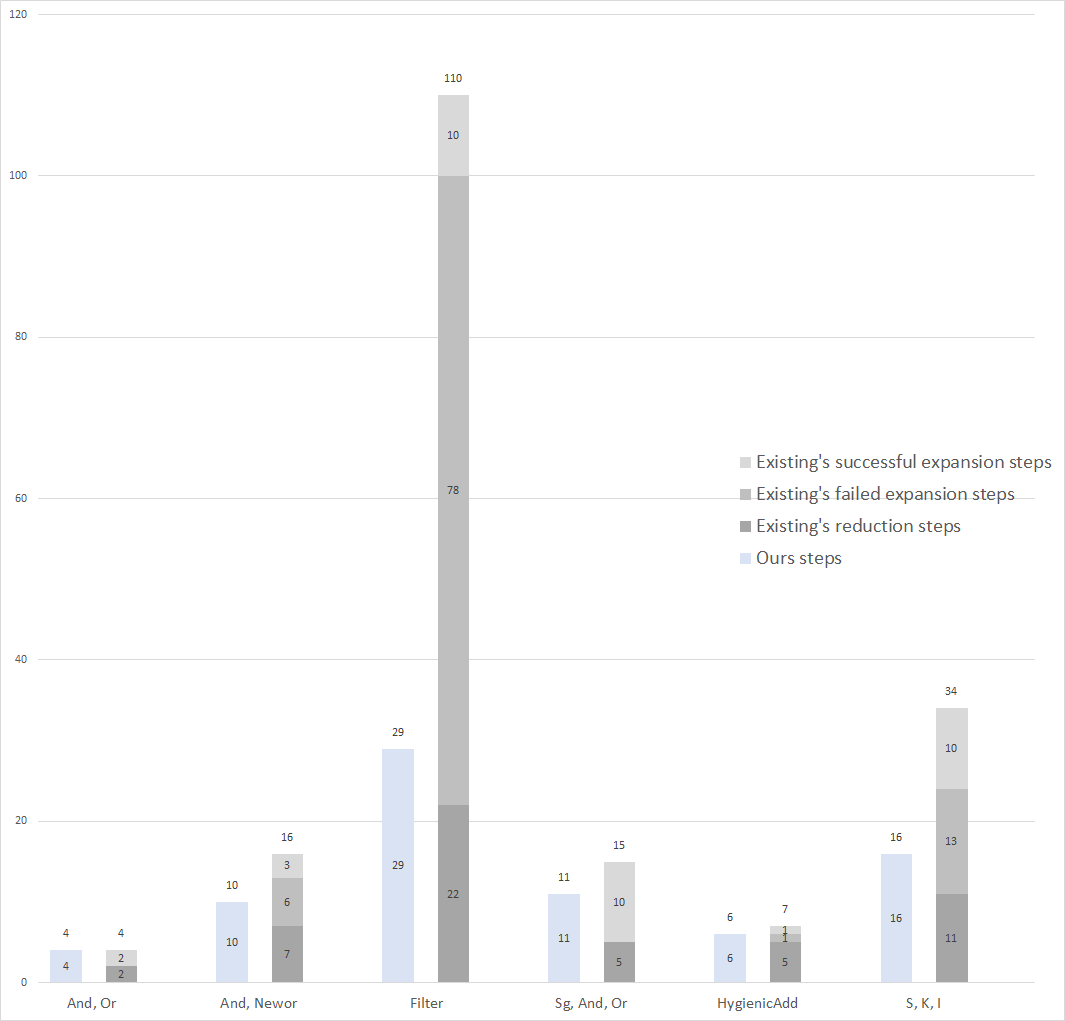
\includegraphics[width=0.48\textwidth]{images/efficiency.png}
	\caption{Comparison on Reduction Steps}
	\label{fig:step}
\end{figure}

To show the efficiency of our approach, we use the number of reduction steps comparing to the existing approach as the metrics. Figure \ref{fig:step} shows the difference between the two approaches. Notice that both approaches have pre-processing---for the existing one, it is to desugar the programs to the core language together with some tags; for ours, it is to calculate the context rules of syntactic sugars. We do not consider the steps during pre-processing. Besides, we derive the reduction steps of the existing approach into three different kinds---the reductions in the core language, the reverse expansion with failed resugaring, the reverse expansion with successful resugaring.  Use the following example to see the difference. Consider a sugar named \m{Hard} with two arguments, which has many reduction steps after desugared. Assuming for specific $e_1$ and $e_2$, the \Code{(Hard $e_1$ $e_2$)} after fully desugared has 100 reduction steps (finally to \#f, for example), and only 1 intermediate step can be resugared (to \Code{(Hard $v_1$ $e_2$)}, for example). Then for \Code{(And (Hard $e_1$ $e_2$) \#t)}, although all the 100 steps in the core language try the reverse desugaring, only \Code{(if stepn \#t \#f)} (2 steps on \m{And}, \m{Hard}) and \Code{(if \#f \#t \#f)} (1 step on \m{And}) are successful. Other 98 attempts will be failed together with 98 steps on \m{And}.

\[
{\footnotesize
	\begin{array}{lcl}
	Surface&&Core\\
	\Code{(And (Hard $e_1$ $e_2$) \#t)}&\xrightarrow{desugar}&\Code{(if step0 \#t \#f)}\\
	\qquad\quad\dashdownarrow& &\qquad\qquad\downarrow\\
	\Code{(And step1 \#t)}&\xleftarrow{resugar}&\Code{(if step1 \#t \#f)}\\
	\qquad\quad\vdots& &\qquad\qquad\vdots\\
	\Code{(And (Hard $v_1$ $e_2$) \#t)}&\xleftarrow{resugar}&\Code{(if stepn \#t \#f)}\\
	\qquad\quad\vdots& &\qquad\qquad\vdots\\
	\Code{(And \#f \#t)}&\xleftarrow{resugar}& \Code{(if \#f \#t \#f)}\\
	\qquad\quad\dashdownarrow& &\qquad\qquad\downarrow\\
	\Code{\#f}&& \Code{\#f}\\
\end{array}
}
\]


The general regularity is---the more complex the sugar is, the more steps will our approach save. Note that if the RHS of a syntactic sugar is huge, one-step reduction of the reverse desugaring will also be complex, because huge sugars will contain many failed attempts to resugar. So avoiding reverse expansion of syntactic sugar can improve the efficiency for practical use because programs are usually not that small like the demos.
